\chapter{Graphcoverage}

Wie zuvor gesehen, existieren verschiedene Coverage-Kriterien um Testabdeckung zu prüfen.
Graphcoverage ist hierbei eine Herangehensweise um graphenbasierte Datenstrukturen zu überdecken.
Graphen können nämlich ähnliche Probleme aufweisen wie vorheriges Beispiel der Addition.
Die Addition zweier 64-bit Integer ist wenigstens endlich, Graphenstrukturen haben sogar unter Umständen unendliche Testräume.
Umso wichtiger ist es hier, dass Überdeckungskriterien formuliert werden können, die diesen möglicherweise unendlichen Suchraum
stark verkleinern und dennoch eine ausreichende Testung ermöglichen.
Da wir vorher ergründet haben, dass GraphQL sich als gerichteten Graph darstellen lässt, können wir nun die Graphcoverage nutzen, um Tests mithilfe der Grapcoverage zu erstellen.
Wie genau die Coverage erstellt wird und daraus Tests resultieren, werden im folgenden geklärt.
Gerichtete Graphen sind die Grundlage für viele Coverage-kriterien, wobei die Grundidee hierbei ist,
Sachverhalte als Graphen zu modellieren und dann eine ausreichende Überdeckung zu finden. \cite[vgl. Software-testing S. 27 2.1]{software-testing}
In $4.1.2$ wurden gerichtete Graphen bereits eingeführt, daher können wir direkt fortfahren und verschiedene
Kriterien definieren, die einen Graphen überdecken.
Wir erklären zuerst verschiedene Techniken, die einen Graphen überdecken und erklären dann ihre Anwendung
an Beispielen.
Erst sortieren wir Graphcoverage ein im Kontext von Code-Coverage und bilden im zweiten Schritt eine Coverage für GraphQL\@.

\section{Graphcoverage allgemein}

Um Graphcoverage zu nutzen, verfeinern wir zuerst die allgemeine Definition von gerichteten Graphen.
Ein gerichteter Graph ist ein Paar $G = (V, E)$ zweier disjunkter Mengen mit $E \subseteq V^2$ wobei alle Elemente aus E gerichtete Kanten sind. [vgl. 4.1.2]
Die Definition erweitern wir nun mit:

\begin{description}
    \item[Menge N] von Knoten
    \item[Menge N_{0}] von Anfangsknoten, wobei N_{0} $\subseteq$ N
    \item[Menge N_{f}] von Endknoten, wobei N_{f} $\subseteq$ N
    \item[Menge E] von Kanten, wobei E $\subseteq$ N x N. Hierbei ist die Menge als init{x} x target{y} definiert.
\end{description}~\cite[2.1 Overview]{software-testing}

Mithilfe dieser Definition können nun zum Beispiel Kontrollflussgraphen abgebildet werden indem die Einstiegspunkte die Anfangsknoten sind und die Endknoten die Austrittspunkte.
Ein Pfad innerhalb von eben definierten Graphen, mit möglicher Länge Null, der in einem Knoten N_{0} startet und in einem Knoten N_{f} endet, nennt sich Testpfad \cite[vgl. S. 28]{software-testing}

\section{Graphcoverage Kriterien}

Mithilfe voriger Definition können wir nun Coveragekriterien entwickeln, die uns Testpfade liefern, die je nach Kriterium für eine spezielle Abdeckung
des Graphens mit Test-Requirements sorgen.

\subsection{Node Coverage}

Node-Coverage ist ein Coveragekriterium, dass alle Knoten, die von $N_{0}$ erreichbar sind, in einem Graphen abdecken soll.
Definieren wir folgenden, sehr einfachen Graphen:

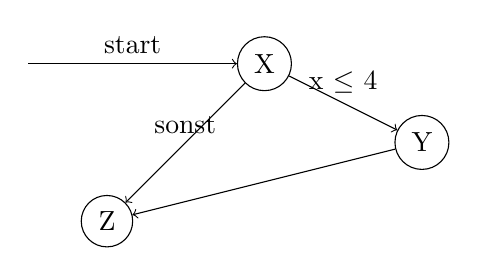
\begin{tikzpicture}
    \node[circle, draw] (n1) at (2,2) {X};
    \node[circle, draw] (n2) at (4,1) {Y};
    \node[circle, draw] (n3) at (0,0) {Z};

    \draw[->] (-1,2) -- node[above] {start} (n1);
    \draw[->] (n1) -- node[above] {x $\le$ 4} (n2);
    \draw[->] (n2) -- (n3);
    \draw[->] (n1) -- node[above] {sonst} (n3);
\end{tikzpicture}

So wäre die Node-Coverage mit einem Test einzigen Test erfüllbar.
Dieser müsste der Pfad $X -> Y -> Z$ sein.
Es ist auch denkbar, dass wir zwei Pfade oder mehr nutzen allerdings erfüllt dieser Pfad schon unser Kriterium daher geben wir uns vorerst zufrieden.
Wir sehen schnell, dass dieser Ansatz noch Lücken aufweist, da der Pfad $X -> Y -> Z$ das Kriterium erfüllt, allerdings wird eine Kante $X -> Z$ nicht im
Test berücksichtigt und kann somit ungetestet bleiben.
Wir führen also noch andere Kriterien ein, die eher geeignet wären.

\subsection{Edge-Coverage}

Edge-Coverage ist ein Coveragekriterium, dass die Kanten in einem Graphen abdecken soll.
Ziel der Edge-Coverage ist es, dass jede Kante des Graphens durch mindestens einen Test abgedeckt wird.
Um die Edge-Coverage für vorheriges Beispiel zu erreichen, benötigen wir schon zwei Routen.
Der Graph:

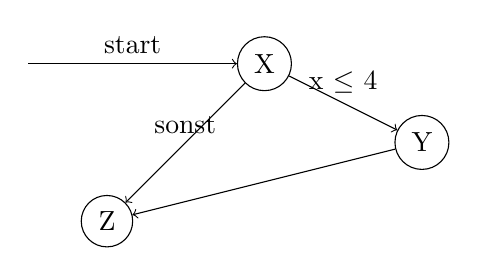
\begin{tikzpicture}
    \node[circle, draw] (n1) at (2,2) {X};
    \node[circle, draw] (n2) at (4,1) {Y};
    \node[circle, draw] (n3) at (0,0) {Z};

    \draw[->] (-1,2) -- node[above] {start} (n1);
    \draw[->] (n1) -- node[above] {x $\le$ 4} (n2);
    \draw[->] (n2) -- (n3);
    \draw[->] (n1) -- node[above] {sonst} (n3);
\end{tikzpicture}

wird über die Pfade $X -> Y -> Z$ und $X -> Z$ überdeckt.
Edge-Coverage hat allerdings auch Probleme Graphen vollständig zu überdecken.
Man nehme folgendes Beispiel:

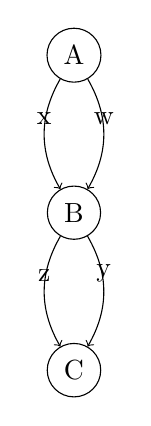
\begin{tikzpicture}
    \node[circle, draw] (a) at (4,4) {A};
    \node[circle, draw] (b) at (4,2) {B};
    \node[circle, draw] (c) at (4,0) {C};

    \draw[->, bend left=30] (a) to node[above] { w } (b);
    \draw[->, bend right=30] (a) to node[above] { x } (b);
    \draw[->, bend left=30] (b) to node[above] { y } (c);
    \draw[->, bend right=30] (b) to node[above] { z } (c);
\end{tikzpicture}

Pfade die laut Edge-Coverage ausreichen um den Graphen zu überdecken wären: \\
$ x \rightarrow z $ \\
$ w \rightarrow y $ \\
Hierbei wird allerdings außer acht gelassen, dass in $x$ auch Änderungen passieren können die Auswirkungen im Programm haben können.
So sind die Routen $ x -> y $ und $ w -> z $ in der Edge-Coverage nicht berücksichtigt.
Allerdings wären diese auch zu testen.
Wir sehen also, dass wir immer noch kein ideales Kriterium gefunden haben.


\subsection{Edge-Pair Coverage}

Das Edge-Pair Coveragekriterium ist eine Erweiterung der Edge-Coverage, indem hier auch die Beziehungen von einzelnen Kanten untereinander berücksichtigt werden um das zuvor
aufgetretene Problem zu lösen.
Ziel dieses Coverage-Kriteriums ist es, dass alle möglichen Kantenpaare abgedeckt sind.





\subsection{Prime-Path Coverage}







\section{Graphcoverage für Code}

\section{Graphcoverage für GraphQL}




